\chapter{Classical Mechanics}

Classical Mechanics describes everything in the world as if they have an exact position $\textbf{x}$ and velocity $\dot{\textbf{x}}$, which in principle could be known simultaneously. There happens to be real physical limit as to how well we can know both of these quantities at the same time (from the Heisenberg Uncertainty principle), but that limit is so small that for everyday objects, Classical Mechanics works just fine.


\section{Lagrangian Formalism}
When dealing with conservative forces, there turns out to be a nice way to figure out all of Newton's laws without having to draw out all of the free body diagrams. In fact, when this method was first proposed, Lagrange bragged that he had \emph{no pictures or diagrams} in his book\footnote{Analytical Mechanics - Lagrange}. The Lagrangian is defined as 
\begin{align}
L\equiv T-V
\end{align}
Where $T$ is the kinetic energy and $U$ is the potential energy. For each coordinate $q_i$ (usually things like $x,y,z$), we get an equation 
\begin{align}
\boxed{\frac{d}{dt}\Big(\frac{\partial L}{\partial \dot{q}_i}\Big) = \frac{\partial L}{\partial q_i} }
\end{align}
These are called the \textbf{Euler-Lagrange equations}. Basically all Classical Mechanics problems boil down to finding a useful set of coordinates to describe your system, then writing out $T$ and $U$ in terms of them, then solving a system of equations given by these.


     An easy way to find the Lagrangian for any system is to identify the coordinate of each of its masses in cartesian coordinates, then rewriting it in terms of coordinates that best suit the problem. 
     \begin{align}
        x_1(q_1,q_2,...)\\
        y_1(q_1,q_2,...)
     \end{align}
     
     We can then just take the time derivative of each of them to solve for the $\dot{q}$ term.




\subsection{Action}\footnote{Following Professor Eric D'Hoker's derivation}
The action is a scalar quantity defined by
\begin{align}
S[q] = \int_{t_1}^{t_2} dt L (q_1,...q_N, \dot{q}_1, ..., \dot{q}_N, t)
\end{align}
The $[q]$ means that it takes as an argument a \emph{function} not just a variable. These types of mathematical objects are called functionals, and take entire trajectories as their argument instead of just one point. In order to find the action, we would have to know exactly the path that $q_1, q_2, q_3, ...$ had all taken, then we integrate the Lagrangian, which is a function of those variables from $t_1$ to $t_2$. 



The importance of the action is that for \emph{any} real physical system, the "path" which all of the coordinates $\textbf{q} = (q_1,q_2,q_3,...)$ follow will be one for which the action will always be at an extremum or saddle point.
\begin{align}
    \frac{\partial S}{\partial \textbf{q}(t)} = 0
\end{align}
This weird fact is called Hamilton's Principle. Apparently the extremization of the action is a direct consequence of the second law of thermodynamics, that entropy is always increasing.\footnote{todo - \url{https://physics.stackexchange.com/questions/47581/entropy-and-the-principle-of-least-action}} Knowing that the integral of the Lagrangian extremizes the Action, we can actually derive Lagrange's equations of motion using variational calculus.

To do so, we consider two possible Lagrangians, one is a function of all of the coordinates that truly minimize the action, $q_1, q_2, q_3, ... $ etc, and one is a set that is infinitesimally close to them $q_1', q_2', q_3', ...$ related by
\begin{align}
    q_i'(t) = q_i(t) + \epsilon s(t)
\end{align}
The differences in the Lagrangians of each case is
\begin{align}
    \delta L(q,\dot{q},t) &= L(q',\dot{q}',t) - L(q,\dot{q},t)\\
\end{align}
Since the difference in the Lagrangian will be small (from the small change in $q$) we can look at the first order in the Taylor expansion of the difference, which is
\begin{align}
    \delta L(q,\dot{q},t) &= \frac{\partial L}{\partial q} \delta q + \frac{\partial L}{\partial \dot{q}}\delta \dot{q}\\
    &\approx \epsilon\Big( \frac{\partial L}{\partial q} s + \frac{\partial L}{\partial \dot{q}}\dot{s}\Big)
\end{align}
Now looking at the change in the action, we have
\begin{align}
    \delta S[q] = \epsilon\int_{t_1}^{t_2} dt \Big( \frac{\partial L}{\partial q} s + \frac{\partial L}{\partial \dot{q}}\dot{s}\Big)
\end{align}
We can integrate the $\dot{s}$ term by parts and find
\begin{align}
    \delta S[q] = \epsilon\int_{t_1}^{t_2} dt \Big( \frac{\partial L}{\partial q}  - \frac{d}{dt}\frac{\partial L}{\partial \dot{q}}\Big)s(t)
\end{align}
If we want the difference in the action between the two paths to be zero (giving us our original path back) and know that $s(t)$ is an entirely arbitrary function, we have to have the integrand be zero
\begin{align}
    \frac{\partial L}{\partial q}  - \frac{d}{dt}\frac{\partial L}{\partial \dot{q}} = 0
\end{align}
These are of course the Euler-Lagrange equations of motion for a system.

%TODO- Also do a simple example where you get back Newton's laws in an easy case


%Equivalent Lagrangians

%$$L(q') = L(q) + \frac{d}{dt}\Lambda(q,t)$$

%For finding equivalent Lagrangians, you will write the new $q'$ as

%$$q'_i = q_i + \epsilon \delta q_i$$

%Using the above equation, you can find that 

%$$\frac{\partial L(q')}{\partial \epsilon}|_{\epsilon = 0} = \sum \frac{\partial L}{\partial q_i}\delta q_i + \frac{\partial L}{\partial \dot{q}_i}\delta \dot{q}_i = \frac{d\Lambda}{dt}$$



\subsection{Holonomic Constraints}
This is essentially when you want to say that a particle must travel along some path, or that the length of a rope is only so long, etc. Basically you can write out the constraint as a formula, lets do the length of a string hanging off a ledge.

\begin{align}
    l = x + z
\end{align}
Which would be if we have the horizontal component of the string given by $x$ and vertical by $z$. Our constraint equation is thus
\begin{align}
    \phi(x,z,t) = 0 = l - x - z
\end{align}
From here, we use Lagrange multipliers (Section \ref{lagrange-mult}) within Lagrange's equations over all our constraints...

$$\frac{d}{dt}\frac{\partial L}{\partial\dot{q}_i} - \frac{\partial L}{\partial q_i} - \sum_\alpha \lambda_\alpha \frac{\partial \phi_\alpha}{\partial q_i} = 0$$

So for each constraint, you have another Lagrange multiplier. To solve for $\lambda_\alpha$ and, and therefore the equations of motion, first look for equations that don't contain the term (i.e. $\partial\phi_\alpha/\partial q_i = 0$), solve those equations, then plug their solution into ones that do, eventually finding them.


You can also solve for one of the coordinates in terms of the other ones in the constraint, and plug it in explicitly to the Lagrangian, then find the E.L. Equations from there.

\subsection{Normal Modes}
The normal modes of a system are when all parts of the system are oscillating with the same frequency. So to solve these, we take the ansatz usually that
\begin{align}
    q_1(t) = Ae^{i\omega t} && q_2(t) = Be^{i\omega t}
\end{align}
Then we can use these in the equations of motion, and solve for the frequencies, usually in a quadratic equation.

\subsection{Equilibrium}

We know that a system is in equilibrium if the forces acting on it are equal to zero. This means that

$$\frac{\partial V}{\partial q_i}|_{q_i=q_i^0} = 0$$

This means that the variable $q_i$ will not be accelerated and is in equilibrium. The equilibrium point can be solved for by calculating this quantity, then solving for what $q_i^0$ must be. We can then find what small oscillations around the equilibrium would be by guessing a solution of the form 

\begin{align}
q_i(t) = q_i^0 + \eta_i(t)  
\end{align}

From here, we just plug this into the Euler-Lagrange equations for $q_i$, and solve for the equations of motion for $\eta(t)$, which tells us how the system moves for small oscillations around an equilibrium.

\subsection{Noether's Theorem}
The essence of what this theorem says is that for every symmetry we can find in our system, there will be some kind of "conserved quantity" associated with it that does not change with time.
Plug in conserved charges in equations of motion, \emph{not} Lagrangian.
$$Q = \sum\frac{\partial L}{\partial\dot{q}_i}\delta q_i - \Lambda$$

$Q$ is a conserved quantity, i.e. $dQ/dt = 0$
Some nice examples of Noether charges are things like the energy of the system, or the angular momentum. 

%TODO Add more here


\subsection{Solving the Equations of Motion}
\begin{enumerate}
    \item Write out the kinetic and potential energies in a nice choice of coordinates.
    \item Find all the Holonomic constraints and plug them in (or do it the other way)
    \item Find EL equations
    \item Find Noether Charges
    \item Plug in Noether charges into EL equations.
\end{enumerate}


\section{Hamiltonian Formalism}
In a way identical to what we do for thermodynamics, we can make a \emph{Legendre transform} of our variables into a new set. We start by defining the canonical momentum as
\begin{align}
p_i \equiv \frac{\partial L}{\partial \dot{q}_i}
\end{align}

$$H = \sum\frac{dL}{d\dot{q_i}}d\dot{q_i} - L$$

\section{Virial Theorem}
Imagine we have some value called $G$ that is defined as
\begin{align}
G = \sum_{k=1}^N \textbf{p}_k\cdot\textbf{r}_k
\end{align}
Where $\textbf{p}_k$ is the momentum of the $k$th particle of $N$, and $\textbf{x}_k$ it's coordinate. It can be shown\footnote{\url{https://en.wikipedia.org/wiki/Virial_theorem}} that this quantity is identical to half the time derivative of the moment of inertia with
\begin{align}
G = \frac{1}{2}\frac{dI}{dt}
\end{align}
The trick to derive the Virial theorem is to take the time derivative of $G$, giving us
\begin{align}
\frac{dG}{dt} &= \sum_{k=1}^N \Big[\textbf{p}_k\cdot\frac{d\textbf{r}_k}{dt} + \frac{d\textbf{p}_k}{dt}\cdot\textbf{r}_k\Big]\\
&= \sum_{k=1}^N \Big[m\frac{d\textbf{r}_k}{dt}\cdot\frac{d\textbf{r}_k}{dt} + \textbf{F}_k\cdot\textbf{r}_k\Big]\\
&= 2T - \sum_{k=1}^N \textbf{F}_k\cdot\textbf{r}_k
\end{align}
The total force on any one particle $\textbf{F}_k$ is given by the sum of all of the individual forces from each of the other particles, or
\begin{align}
\textbf{F}_k = \sum_{j\neq k}^N \textbf{F}_{jk}
\end{align}
This lets us rewrite the second term as
\begin{align}
\sum_{k=1}^N \textbf{F}_k = \sum_{k=1}^N \sum_{j\neq k}^N \textbf{F}_{jk}\cdot\textbf{r}_k = \sum_{k=1}^N \sum_{j\neq k}^N \textbf{F}_{jk}\cdot(\textbf{r}_k - \textbf{r}_j)
\end{align}
Where the last bit is kosher because no particle has a self force or $\textbf{F}_{jj} = 0$. The usefulness of the theorem come when we have a potential between each particle is a power series of the form $V(\textbf{r}_k - \textbf{r}_j)  = \alpha |\textbf{r}_j-\textbf{r}_k|^n$, since
\begin{align}
\textbf{F}_{jk}\cdot(\textbf{r}_k - \textbf{r}_j) = \Big[-\nabla_k V(\textbf{r}_k - \textbf{r}_j) \Big]\cdot(\textbf{r}_k - \textbf{r}_j) = n V(\textbf{r}_k - \textbf{r}_j) 
\end{align}
Therefore
\begin{align}
n \sum_{k=1}^N \sum_{j\neq k}^N V(\textbf{r}_k - \textbf{r}_j) = nV
\end{align}
Where $V$ is the total potential energy of the system. Therefore if we look at the average, and have a \emph{stably bound system} we have that
\begin{align}
\Big\langle\frac{dG}{dt}\Big\rangle = 0 = 2\langle T \rangle - n\langle V \rangle 
\end{align}
Where $n$ of course is the power of the potential.


%TODO \section{Hamilton-Jacobi Equations}
%Someday...

\section{Special Relativity}
It turns out that both space and time get jumbled together when you move fast enough. Special relativity is able to talk about two frames (i.e. two people) which move at a constant velocity with respect to one another. The theory was developed as a consequence of the strange fact that the speed of light, found in Maxwell's equations, was found to be \emph{completely independent} of whatever frame you are in. 

\centerline{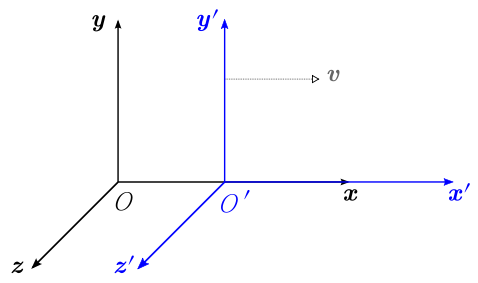
\includegraphics[width=0.5\textwidth]{physics/images/relativity}}

With relativity, we always talk about "frames" which are just places that you, as an observer would see things from. Galilean relativity (or "common sense" relativity) says that if you have light of speed $c$ in one frame $F$, which is moving at speed $v$ towards an observer in frame $F'$, the speed of light should be 
\begin{align}
    c' = v+ c
\end{align}
If for instance the like was going towards the origin $O$ in frame $F$. This would be \emph{faster} than what Maxwell's equation's say, so something has to give. Einstein fixed this by positing that both \emph{space and time themselves} are changed between frames with different velocities. When you look at something that is moving, it is shrunken in the direction of travel compared to how it sees itself. Additionally the amount of time it takes for an event to take place (ball thrown, clock tick, etc) takes \emph{longer} in the frame that sees the event as moving, than it would in a frame at which the the event takes place at rest. 


To illuminate, lets pretend we have a person on earth (frame $F$) and a person on a spaceship (frame $F'$) moving away from the earth in the positive $x$ direction with speed $v$. The earth measures everything with coordinates $(t,x,y,z)$ and the person on the ship measures everything with coordinates $(t',x',y',z')$. Both of these coordinate systems are \emph{completely normal} in their own frames. If they had a ball on earth and measured it's radius as $r$, the ruler with which they measure it on the ship would say it is the same $r$ when the entire ship, ball, ruler system is moving together. 

Lets pretend that right when the spaceship passes the earth, they are able to align their coordinate system somehow so everything is zero. The usefulness of special relativity is know how everyone on the ship (in $F'$) sees things after doing some mathematics with all of the things you are capable of measuring in $F$. It turns out that the transformation is given by \footnote{do someday, classical HW 3}
\begin{align}\label{lorentzcontract}
    t' &= \gamma\Big(t -\frac{vx}{c^2} \Big)\\
    x' &= \gamma(x - vt)\\
    y' &= y\\
    z' &= z
\end{align}
Where 
\begin{align}
\gamma =\frac{1}{ \sqrt{1-\frac{v^2}{c^2}}  }
\end{align}
% TODO We can remember these equations as follows. In Galilean relativity, after drawing out the frames, we would have
%\begin{align}
%   x' = x - vt
%\end{align}
%Both are modulated by $\gamma$, to keep the expression finite when $v$ gets larger and larger. The sign on the time matches $x$, and must match units and $t$. ...  TODO

We can do something interesting from here, lets look at the following quantity
\begin{align}
    s^2 &= -c^2t'^2 +x'^2 + y'^2 + z'^2\\
    &= \frac{c^2(t^2 - \frac{vx}{c^2})^2}{1-\frac{v^2}{c^2}}  + \frac{(x - vt)^2}{1-\frac{v^2}{c^2}} + y^2 + z^2\\
    &= -c^2t^2 + x^2 + y^2 + z^2
\end{align}
It turns out this quantity is \emph{invariant} when we change between frames. These type of things are incredibly important when dealing with topics in special relativity

\subsection{Four Vectors}
A nice way to write things that give us invariants easily is in four vector notation. We can define the position \emph{contravariant} vector with
$$ x^\mu \equiv (x^0, x^1,x^2,x^3) = (ct,x,y,z) $$
Remember the signs by knowing all the vectors with \textit{upper} indices have all \textit{positive} quantities. We can then define a \emph{covariant} with
\begin{align}
     x_\mu \equiv (-x^0, x^1,x^2,x^3) = (-ct,x,y,z) 
\end{align}
We see that if we dot these two vectors we get 
\begin{align}
    s^2 = x_\mu x^\mu = -c^2t^2 + x^2 + y^2 + z^2
    \end{align}
This one tells us things about how events are causally connected to one another, since

$$s^2 = - c^2(t_2-t_1)^2 + (\textbf{x}_2-\textbf{x}_1)^2$$

\begin{itemize}
\item $s^2 = 0$ Lightlike, only massless particles moving at $c$ will have this 0 
\item $s^2 > 0$ Spacelike, in every frame, there will always be some separation of space between the events. Causally unrelated
\item $s^2 < 0$ Timelike, time separates these events in all frames.
\end{itemize}

Another useful thing that comes up often is the \textbf{Minkowski Metric} defined as 

\begin{align}
\eta_{\mu\nu} = \left(
{\begin{array}{cccc}
-1&0&0&0\\
0&1&0&0\\
0&0&1&0\\
0&0&0&1
\end{array}}
\right)
\end{align}
This transforms a contravariant into a covariant with
\begin{align}
    x_\mu = \eta_{\mu\nu}x^\nu
\end{align}
Also important is the 4-gradient

\begin{align}
\partial_\mu &\equiv \frac{\partial}{\partial x^\mu} = (\frac{\partial t}{\partial x^0}\frac{\partial}{\partial t}, \frac{\partial x}{\partial x^1}\frac{\partial}{\partial x}, \frac{\partial y}{\partial x^2} \frac{\partial}{\partial y},\frac{\partial z}{\partial x^3}\frac{\partial}{\partial z} ) = (\frac{1}{c} \partial_t, \partial_x,\partial_y,\partial_z)
\end{align}

Be aware that the lower index partial is with respect to the upper index $x$. Similarly this gives
$$\partial^\mu = (-\frac{1}{c}\partial_t,\partial_x,\partial_y, \partial_z)$$

\subsection{Relativistic Kinematics}
The key equation to remember is 
\begin{align}\label{relenergy}
    E^2 = p^2c^2 +m^2c^4
\end{align}
We can define the \emph{four momentum} as
\begin{align}
    p^\mu = (E/c,p_x,p_y,p_z)
\end{align}
Notations can sometimes swap the minus signs, but it seems easier to remember that all raised index vectors are entirely positive. The covariant is the same with the front sign swapped. We see that if we rearrange equation \ref{relenergy} we can find
\begin{align}
- m^2c^2 = -\frac{E^2}{c^2} + p^2 = p_\mu p^\mu
\end{align}
Usually in the problems here you are given two objects with momentum $p_1^\mu$ and $p_2^\mu$ respectively, that turn into a new particle with four-vector $p_3^\mu$. We know that in general
\begin{align}
    p_3^\mu = p_1^\mu + p_2^\mu
\end{align}
Which means we just add each of the components of the vector like normal, which gives us the new 4 momentum. From here, we can find the invariant mass of the system just doing
\begin{align}
    -m_3^2c^2 = (p_{1\mu} + p_{2\mu})(p_1^\mu + p_2^\mu)
\end{align}
Proper time is Lorentz invariant and defined as

\begin{equation}\label{propertime}
c^2d\tau^2 = -\eta_{\mu\nu}dx^{\mu}dx^{\nu}
\end{equation}
The 4-velocity is then defined as

$$u^\mu \equiv \frac{d x^\mu}{d\tau}$$
Plugging in our definition back into equation \ref{propertime} we get that 
\begin{align}
-c^2 &= u_\mu u^\nu\\
 &= -c^2\frac{d t}{d \tau}^2 + \frac{d x}{d \tau}^2 + \frac{d y}{d \tau}^2 + \frac{d z}{d \tau}^2\\
 &= -c^2\frac{d t}{d \tau}^2(1- \frac{v^2}{c^2}) 
\end{align}
This gives us time dilation with $\gamma d\tau = dt$. Replugging this into the definition of the 4-velocity, we get

$$u^\mu = (\gamma c, \gamma v_x, \gamma v_y,\gamma v_z)$$
This allows us to then define the 4-momentum of a massive particle as 
$$p^\mu \equiv mu^\mu = (\gamma mc, \gamma mv_x, \gamma mv_y,\gamma mv_z)$$
The Lorentz force equation is given by

$$\frac{dp^\mu}{d\tau} = eF^{\mu\nu}\frac{dx^\nu}{d\tau}$$


There is a similar way to write the boost in momentum and energy as we did for space and time
\begin{align}
    E' &= \gamma(E - vp_x)\\
    p_x' &= \gamma(p_x - vE/c^2)\\
    p_y' &= p_y\\
    p_z' &= p_z
\end{align}
If the other frame $F'$ is moving with velocity $v$ in the $x$ direction relative to frame $F$.


\section{Rotation}\label{classicalrot}



\begin{figure}\label{rotation}
\centerline{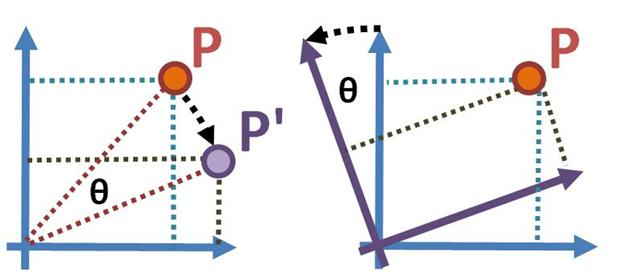
\includegraphics[width=0.7\textwidth]{physics/images/rotation}}
\caption{The left is an \emph{active} rotation, which involves physical rotation of an object. The right is a \emph{passive} rotation which involves instead the rotation of the coordinate system.}
\end{figure}

$$R(\hat{n},\theta)$$

$R$ is a rotation matrix, $\hat{n}$ is what axis you are choosing to rotate around, points along that axis. $\theta$ determines how far around that axis you are going to rotate. Directions are chosen from the cross product, for instance if it is $\hat{z}$, we know $x\times y=z$, so that requires use to have it such that it looks like $x$ chases $y$, or $x$ will move towards $y$ in the direction it is closest to it from. This turns out to happen for all of the pairs, when said in order, i.e.

\begin{align}
x\times y &= z\\
y\times z &= x\\
z\times x &= y\\
\end{align}

If you ever find them in the opposite order, it is equivalent to going the opposite direction. There are two typical conventions for rotations outline in Figure \ref{rotation}. In most cases, we only care about the active rotation, given around the $\hat{z}$ axis below with

\begin{align}
R(\hat{z},\theta) =  \left(
{\begin{array}{ccc}
\cos\theta&-\sin\theta&0\\
\sin\theta&\cos\theta&0\\
0&0&1\\
\end{array}}
\right)
\end{align}

Similar rotations around $\hat{x},\hat{y}$ can be found easily by cyclically permutating the vectors and realigning, with

\begin{align}\left(
{\begin{array}{c}
x_1\\
y_1\\
z_1\\
\end{array}}\right) &\rightarrow
\left(
{\begin{array}{c}
z_1\\
x_1\\
y_1\\
\end{array}}\right) \\
\left(
{\begin{array}{c}
z_1'\\
x_1'\\
y_1'\\
\end{array}}\right) &= 
\left(
{\begin{array}{ccc}
\cos\theta&-\sin\theta&0\\
\sin\theta&\cos\theta&0\\
0&0&1\\
\end{array}}
\right)\left(
{\begin{array}{c}
z_1\\
x_1\\
y_1\\
\end{array}}\right)\\
\rm{Reorder}\implies  
\left(
{\begin{array}{c}
x_1'\\
y_1'\\
z_1'\\
\end{array}}\right)
&= \left(
{\begin{array}{ccc}
\cos\theta&0 &\sin\theta\\
0&1&0\\
-\sin\theta&0&\cos\theta\\
\end{array}}
\right)\left(
{\begin{array}{c}
x_1\\
y_1\\
z_1\\
\end{array}}\right)
\end{align}
This is a rotation around the $\hat{y}$ axis, as that direction is unaffected. 




\subsection{Rotating Frames}
Given a rotating frame $r$ which is rotating with constant angular velocity $\omega$ and we want to find a non-rotating frame $s$ where Newton's laws apply, we have that
\begin{align}
\textbf{v}_s = \textbf{v}_r + \boldsymbol{\omega}\times\textbf{r}
\end{align}
Where $r$ is the distance from the center of rotation. To find the acceleration, we must also consider the unit vectors as a function of time, with %\todo{Fix this, do in index notation}
\begin{align}
\textbf{a}_s = \frac{d\textbf{v}_s}{dt} &= \frac{d}{dt}\Big[|v_x|\hat{x} + |v_y|\hat{y} + |v_z|\hat{z} + \boldsymbol{\omega}\times(|r_x|\hat{x} + |r_y|\hat{y} + |r_z|\hat{z})\Big]\\
&= \Big[|\dot{v}_x|\hat{x} + |\dot{v}_y|\hat{y} + |\dot{v}_z|\hat{z} + \boldsymbol{\omega}\times(|\dot{r}_x|\hat{x} + |\dot{r}_y|\hat{y} + |\dot{r}_z|\hat{z})\Big] \\
&+ \Big[|v_x|\dot{\hat{x}} + |v_y|\dot{\hat{y}} + |v_z|\dot{\hat{z}}  +\boldsymbol{\omega}\times(|r_x|\dot{\hat{x}} + |r_y|\dot{\hat{y}} + |r_z|\dot{\hat{z}})\Big]\\
\end{align}
In general the time derivative of any unit vector in a rotating frame is given by
\begin{align}
\dot{\hat{u}} = \boldsymbol{\omega}\times\hat{u}
\end{align}
We also know that $\dot{r}_i = v_i$ and $\dot{v}_i = a_i$ since they are simply the rate of change of the objects position and velocity. Thus we have
\begin{align}
\textbf{a}_s &= \textbf{a}_r + \boldsymbol{\omega}\times\textbf{v}_r + \boldsymbol{\omega}\times\textbf{v}_r + \boldsymbol{\omega}\times(\boldsymbol{\omega}\times\textbf{r})\\
&= \textbf{a}_r + 2\boldsymbol{\omega}\times\textbf{v}_r + \boldsymbol{\omega}\times(\boldsymbol{\omega}\times\textbf{r})
\end{align}
Now we care about how Newton's laws look in the rotating frame, and rearranging tells us that
\begin{align}
\textbf{a}_r = \textbf{a}_s - 2\boldsymbol{\omega}\times\textbf{v}_r - \boldsymbol{\omega}\times(\boldsymbol{\omega}\times\textbf{r})
\end{align}
So we have the normal acceleration that would be created from Newton's second law in a non-rotating frame, then two extra terms which are caused by the rotation of the frame itself. The first term is the Coriolis acceleration, and the second is centrifugal acceleration.


\subsection{Moment of Inertia}
To find the moment of inertia of a simple object positioned in a difficult way, first find the moment of inertia of the body in it's center of mass frame such that the tensor is diagonal such that 

$$ I_{CM} = 
\left(
{\begin{array}{ccc}
I_{xx}&0&0\\
0&I_{yy}&0\\
0&0&I_{zz}\\
\end{array}}
\right)$$

With this you can then rotate the tensor to find what it would be if the object is spun on a more difficult axis. with 

$$I_{Rot} = R(\theta_x)R(\theta_y)R(\theta_z)~I_{CM}~R(\theta_z)^{-1}R(\theta_y)^{-1}R(\theta_x)^{-1}$$

If the axis is still not where you want it to be, just apply the parallel axis theorem to again shift it with

$$I_{F} = I_{Rot} + Md^2$$





\section{Fluid Mechanics}
Fluid Mechanics is right on the border of being classical mechanics and statistical mechanics. It has to do with how a large number of particles move together. Looking at the mass density $\rho$, because we cannot create or destroy mass classically, we have
\begin{equation}\label{masscon}
\frac{\partial\rho}{\partial t} = -\nabla\cdot (\rho\textbf{v})
\end{equation}
Which is just the continuity equation, and says that the rate at which the mass density is shrinking is equal to how much mass is leaving each surface at a given time. We also define the momentum of a system by adding up each infinitesimal mass and multiplying it by its respective velocity. This is the same thing as 
\begin{align}
    \textbf{p}(V,t) = \int_V dx^3 \rho(\textbf{x},t)\textbf{v}(\textbf{x},t)
\end{align}
An important thing to note is that the velocity $\textbf{v}$ in the integral is not specifically the velocity of any one particle, but called a \emph{velocity field} since it is defined over the entire volume, and the particles are too small for us to be concerned about any of them individually. Newton's third law tells us that $\textbf{F} = \dot{\textbf{p}}$, so we first define the \emph{force field}
\begin{align}
    \textbf{F}(V,t) = \int_V dx^3 \textbf{f}(\textbf{x},t)
\end{align}
Let's match Newton's third law and find
\begin{align}
    \int_V dx^3 \textbf{f}(\textbf{x},t) &= \frac{d}{dt}\int_V dx^3 \rho(\textbf{x},t)\textbf{v}(\textbf{x},t)
\end{align}
Conservation of momentum (also called Euler's equations) gives us
\begin{equation}\label{momcon}
\rho\left({\frac{\partial\textbf{v}}{\partial t} + (\textbf{v}\cdot\nabla)\textbf{v}}\right) = \textbf{f}
\end{equation}
%TODO Some more trivia
%
%\begin{itemize}
%\item Ideal Fluids
%\begin{itemize}
%\item Force field given by $\textbf{f} = -\nabla p$
%\item Isentropic Flow
%\begin{itemize}
%\item Kelvin's Theorem $\frac{d}{dt}\oint \delta\textbf{x}\cdot\textbf{v} = 0$
%\end{itemize}
%\end{itemize}
%\item Incompressible Fluids -  ($\rho=$ const, $\nabla\cdot \textbf{v} = 0$)
%\item Steady Flow -  $d\textbf{v}/dt = 0$
%\item Potential Flow $\textbf{v} = \nabla\phi$
%\end{itemize}
%If any coordinate goes to infinity ($\textbf{v}\cdot\nabla)\textbf{v} = 0$
%

%\section{TODO}

%\begin{itemize}

%\item Classical HW6 Problem 1, coupled oscillators
%\end{itemize}

